\documentclass{article} % For LaTeX2e
\usepackage{nips13submit_e,times}
\usepackage{hyperref}
\usepackage{url}
\usepackage{graphicx}
\usepackage{amsmath}


\title{Predicting mental functions from brain activations}


\author{
Madhura Parikh\\
Department of Computer Science\\
University of Texas, Austin\\
\texttt{mparikh@cs.utexas.edu} \\
\And
Subhashini Venugopalan \\
Department of Computer Science\\
University of Texas, Austin\\
\texttt{vsubhashini@utexas.edu} \\
}

% The \author macro works with any number of authors. There are two commands
% used to separate the names and addresses of multiple authors: \And and \AND.
%
% Using \And between authors leaves it to \LaTeX{} to determine where to break
% the lines. Using \AND forces a linebreak at that point. So, if \LaTeX{}
% puts 3 of 4 authors names on the first line, and the last on the second
% line, try using \AND instead of \And before the third author name.

\newcommand{\fix}{\marginpar{FIX}}
\newcommand{\new}{\marginpar{NEW}}

%\nipsfinalcopy % Uncomment for camera-ready version

\begin{document}


\maketitle

\begin{abstract}
Over the past few decades neuroscientists have studied brain images from EEG/MEG, fMRI and other sources to identify associations between psychological tasks and activity in brain regions~\cite{PMSKBY12}.
Although these studies have led to large amounts of literature and several discoveries of cognitive functions associated with certain brain regions (or networks) the mapping between functions to brain regions and vice-versa still remains largely unclear. For the purposes of this project, we look at enhancing a new automated framework NeuroSynth~\cite{yarkoni2011large}  that combines text-mining and machine learning techniques to generate probabilistic mappings between cognitive and neural states. Starting from their Naive Bayes classifier, we apply more sophisticated binary classifiers to the problem and also consider multi-label predictions and transfer-learning(?).
\end{abstract}

\section{Introduction and Related work}
In this project, we build on the existing NeuroSynth framework~\footnote{\protect \url{neurosynth.org}}. While the NeuroSynth framework offers tools for several types of meta-analyses, we primarily address the problem of Reverse Inference.  This can be stated more precisely as: \emph{Given a signature of neural activity,  identify  the cognitive state(s) and functions that the activations correspond to} (see fig~\ref{fig:revinf}). The scientific community typically uses fMRI scans for reporting this neural activity. Reverse inference is an extremely challenging problem since multiple cognitive states could have very similar neural signatures~\cite{yarkoni2011large} but it is also of major interest to the neourimaging community at large.

\begin{figure}[h]
\begin{center}
%\framebox[4.0in]{$\;$}
%\fbox{\rule[-.5cm]{0cm}{4cm} \rule[-.5cm]{4cm}{0cm}}
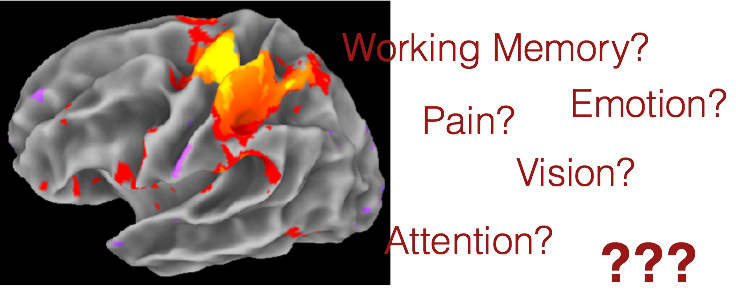
\includegraphics[height=4cm]{revinf.png}
\end{center}
\caption{The reverse inference problem}
\label{fig:revinf}
\end{figure}

Forward and reverse inference problems have been addressed by several contemporary works~\cite{schwartz2013mapping, PMSKBY12, sanmi2013multi, yarkoni2011large}. Previous approaches have generally tackled the Reverse Inference problem by manually analyzing fMRI scans of subjects, collected from the laboratory. There are several limitations of such an approach - for instance, involving human subjects for fMRI scans is labor and cost intensive and the number of data samples that can be gained from such efforts is also very less. Moreover all the meta-analyses based on such data is carried on a very small-scale at individual research labs, and fails to take advantage of the vast knowledge embodied in the entire research community. 

NeuroSynth's (and therefore our) approach is unique - in that we tackle the Reverse Inference problem not by requiring actual fMRI scans, but rather by exploiting the relatively large repository of neuro-imaging publications using text-mining and machine learning techniques.  There are many motivations and benefits that lead to this. For one, while fMRI scans are very few, there has been a growing body of publications related to neuro-imaging, thus offering a much larger source of data. Further by using machine learning techniques the decoding is possible without any real training data (fMRI scans) and at the same time incorporates the knowledge base derived from several researcher. Also to the best of our knowledge, this is the first approach that is fully automated, thus making it possible to perform several meta-analyses on a much larger scale than could ever be possible by individual researchers.  In the next few paragraphs, we introduce the NeuroSynth framework and some of the techniques it utilizes.

\subsection{The NeuroSynth framework}
The figure~\ref{fig:3steps} gives a high-level view of  NeuroSynth. 

\begin{figure}[h]
\begin{center}
%\framebox[4.0in]{$\;$}
%\fbox{\rule[-.5cm]{0cm}{4cm} \rule[-.5cm]{4cm}{0cm}}
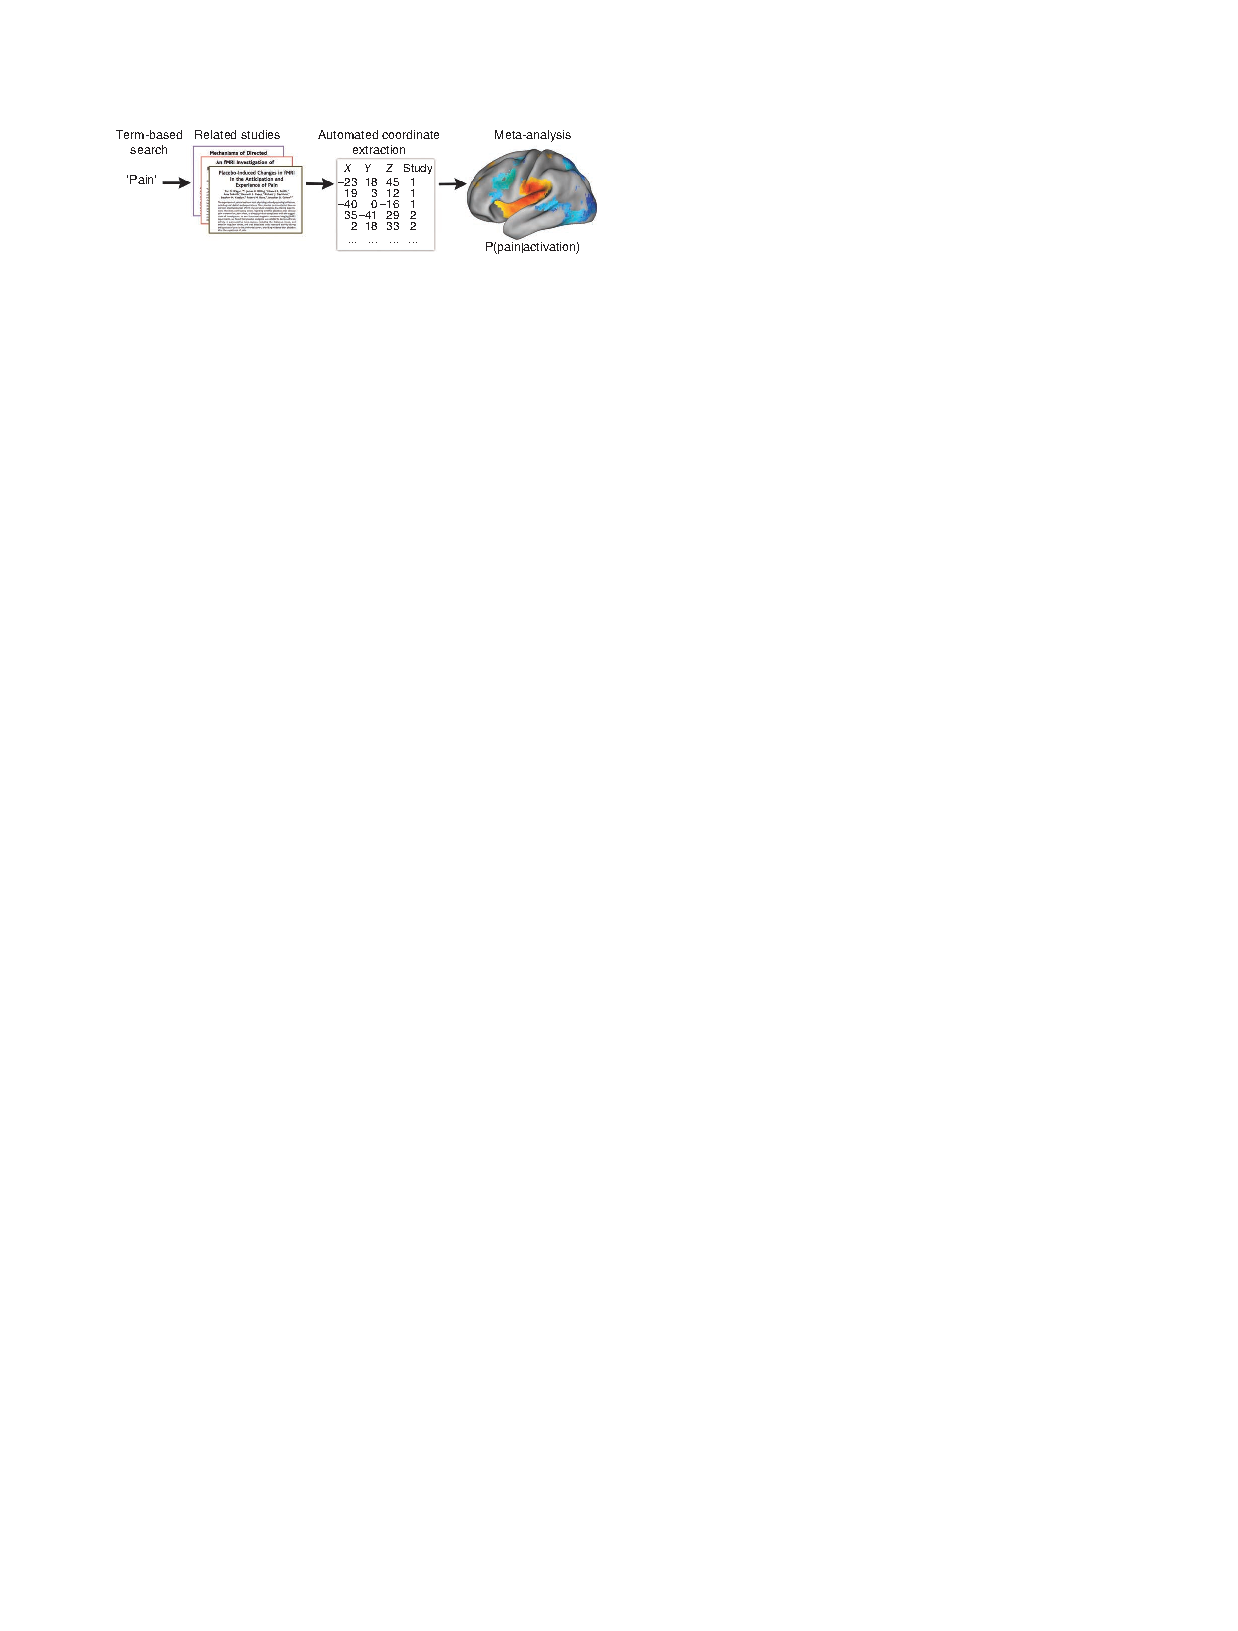
\includegraphics[height=4cm, width=14cm]{3steps.pdf}
\end{center}
\caption{The NeuroSynth framework~\cite{yarkoni2011large}}
\label{fig:3steps}
\end{figure}

A detailed description of NeuroSynth may be found in ~\cite{yarkoni2011large}. Here we give only a high-level view  - figure~\ref{fig:3steps}.  For reverse inference, NeuroSynth performs the following three steps:
\begin{description}
\item[Step 1:  Extract high frequency terms] First, a database of nearly $3000$-odd ~\footnote{The number has grown to over $8000$, since 2011 when ~\cite{yarkoni2011large} was published.} studies is scrapped to extract the most frequent terms and their frequency of occurence across these studies. Thus corresponding to each study we get a set of terms. These set of terms serve as labels for that study, during the classification.
\item[Step 2: Extract coordinates of activation foci and synthesize sparse image] Using simple template matching, all probable activation foci mentioned in a study are extracted. Once we have a list of these coordinates, corresponding to each study, they are used to synthesize extremely sparse brain images with the corresponding brain regions activated. After some preprocessing (which we describe in detail in section~\ref{sec:preprocess}) the vectorized image serves as the feature vector for that study.
\item[Step 3: Use classification to build a predictive model]  Use classification to train a model, give the labels and the feature vectors from steps (1) and (2). They use an extremely simple approach in which they apply a Naive Bayes classifier to make single-label predictions . They pick up $25$ of the most frequent terms arbitarily and train $25 \choose 2$ models (i.e one-vs-one) corredponding to every term pair and 10-fold cv to make the predictions.
\end{description}

There have been other approaches that have further built on NeuroSynth. For instance in ~\cite{sanmi2013multi}, the authors use label decomposition techniques in a one-vs-all setting to predict multiclass labels for the reverse inference problem. They use Support Vector Machines ($l_2$ regularized), logistic regression and ridge classifier for these tasks,  comparing the outcomes based on different criteria like precision, recall and Hamming loss, to show that the multiclass approach is effective for reverse inference. They also propose to use other multiclass approaches and regularization techniques and analyze their performance as future work. 

In another similar work~\cite{schwartz2013mapping} uses a Generalized Linear Model(GLM) for forward inference. For the reverse inference they use logistic regression with Ward clustering to counter the high dimensionality of the problem. 

Building up on these approaches,  in the following sections, we shall describe our own extensions and experiments toward building a better model for the reverse inference problem.

Similar to ~\cite{yarkoni2011large}, we primarily use the repository available with NeuroSynth for our project. This has nearly $8067$ studies that are scrapped from online resources, spanning $15$ journals. For our transfer-learnign approach, we would like to use real fMRI scans, and adapt our models tuned with the synthesized data on this real data. We use data from 2 sources. We use the open source openfMRI~\footnote{\protect \url{https://openfmri.org}} project ~\cite{poldrack2013toward} to gain the training data. This has individual subject level images for $26$ contrasts, resulting in a total of $479$ data samples. Since it is always more advisable to work with group level statistics, we also consider the NeuroVault\footnote{\protect \url{http://neurovault.org}} data that has 17 studies, but with group level images. Ideally we would have liked to use this data entirely but the major issues is that it is too less to be meaningful on its own. 
\subsection{Pre-processing}
\label{sec:preprocess}
Here we describe mainly the preprocessing pipe for the NeuroSynth data. The code repository for NeuroSynth already has the labels and coordinates that are extracted from the $8000$ studies. Beginning with this, we used various open source toolkits like NumPy tand existing utiliities in NeuroSynth to synthesize images corresponding to the the activated coordinates. 

\begin{description}
\item[Step 1: ] First for each $(x, y, z)$ coordinate extracted from a study, we transformed it to the MNI space - which is the standard space used for neuro-imaging. 
\item[Step 2: ] Second, since the coordinates were extracted using simple template matching, there would likely be some spurious numbers that were mistaken as coordinates. It is also possible that the study mentioned coordinates for some different region other than the brain. To deal with such anomalies, we then applied a 2mm MNI mask on the coordinates, to validate that they indeed lay in the brain space and discarded the invalid ones. The 3D mask has the shape $(91 x 109 x 91)$ 
\item[Step 3: ] Since each study mentions only a very few coordinates from the entre brain space, the resulting image we would get would be extremely sparse. Based on connectivity and correlation amongst the brain regions, given an activated focus, it is highly likely that the voxels in its neighbourhood would be actvated as well. Using this fact we considered all voxels in a $6$ mm radius around the activated foci to also be activated and thus get a more dense and smoother image.
\item[Step 4: ] Once we get this synthesized image in $3$D MNI space, we reshape it to a $1$D vector, further removing all zero-columns, to end up with a $1 x 228453$ feature vector.  
\end{description}

Since the data is extracted based on simple text processing, there will likely be irrelevant data that is also included. To deal with this we apply some further steps, in which we only consider terms that have a normalized frequency count $ > 0.001$. Further we only consider those studies to be valid, that have atleast 500 activated voxels in the final feature vector. Further for single-label classification we only consider studies, that have a unique label with normalized frequency  $ > 0.001$. Studies that have multiple labels at a frequency $ > 0.001$ cannot e clearly assigned a single correct label, and we therefore do not consider them for the single-label classification problem.

For the sake of comparibility, we use the same $22$ terms as labels for our experiments as~\cite{yarkoni2011large}\footnote{The paper actually considers $25$ terms however, $3$ of these were absent in the version of the data we worked with} . After we perform the filtering steps we mentioned above, we end up with a total of $2464$ studies out of the original $8067$ studies, for the single label classification task.

For the multi-label classification, we perform the same filtering and pre-processing as mentioned above, the only difference being that this time we allow multiple labels per study, instead of removing the studies with conflicting labels. Thus we end up with a total of $5463$ studies from the original $8067$ studies. Similar to ~\cite{sanmi2013multi} we plot a histogram that shows the distribution of terms across studies (fig~\ref{fig:histo_old}). 

\begin{figure}[h]
\begin{center}
%\framebox[4.0in]{$\;$}
%\fbox{\rule[-.5cm]{0cm}{4cm} \rule[-.5cm]{4cm}{0cm}}
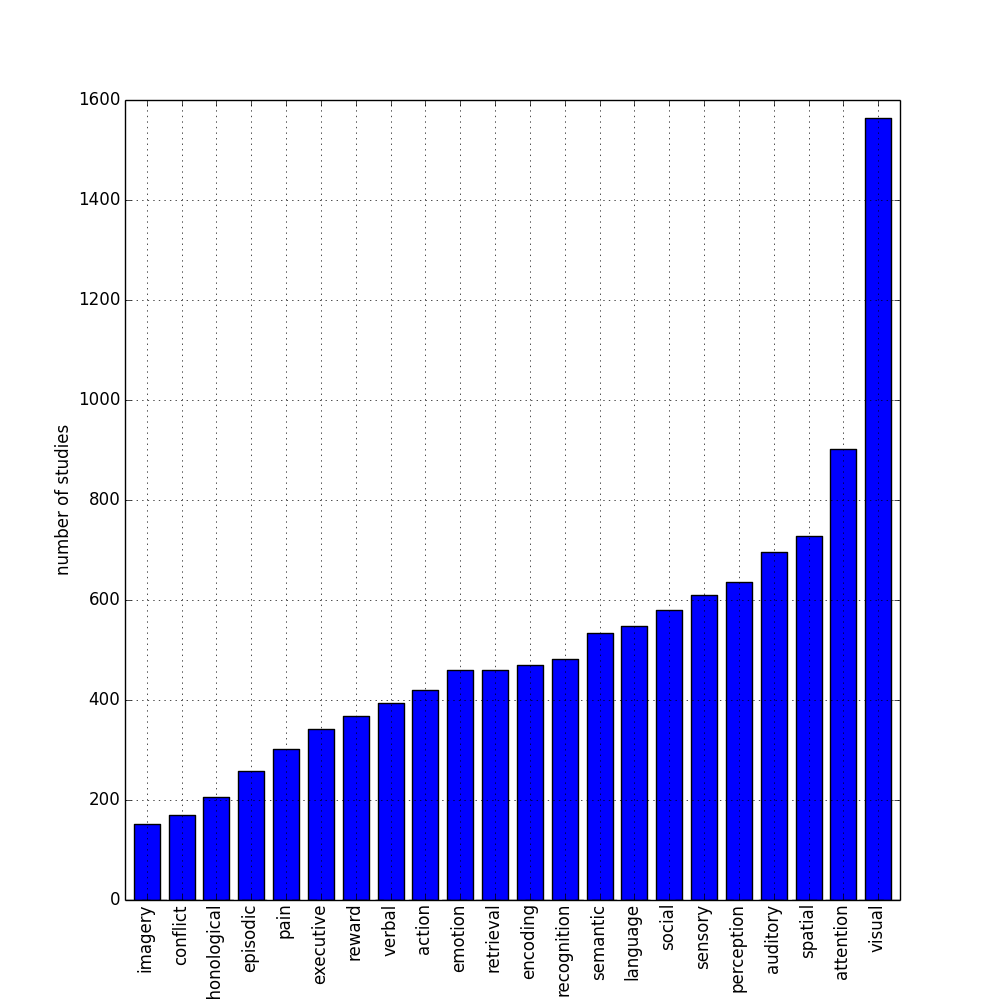
\includegraphics[height=10cm, width=10cm]{histo_old.png}
\end{center}
\caption{\textbf{Distribution of terms across studies:} The x-axis denotes eac term and the y-axis denotes the number of studies in which the term appears.}
\label{fig:histo_old}
\end{figure}

For the purposes of transfer learning we use the openfMRI and NeuroVault repositories as a source of real fMRI data. The openfMRI data is also in a similar format to the NeuroSynth data.  Thus there is a study associated with an fMRI image and these have already been text-processed previously, to give a frequency count for some $19$ terms of interest.  One issue is that the labels in NeuroSynth do not overlap the labels that were extracted for openfMRI. Thus we pick out terms tha would be similar to the openfMRI terms from the NeuroSynth database. Now using these new $19$ terms, we perform a simialr preprocessing as in the multi-label case to filter out studies that would be reliable for these new terms of interest. We end up with $4066$ such studies from the NeuroSynth database. Again a distribution of different terms across the studies is presented in fig~\ref{fig:histo_new}.

\begin{figure}[h]
\begin{center}
%\framebox[4.0in]{$\;$}
%\fbox{\rule[-.5cm]{0cm}{4cm} \rule[-.5cm]{4cm}{0cm}}
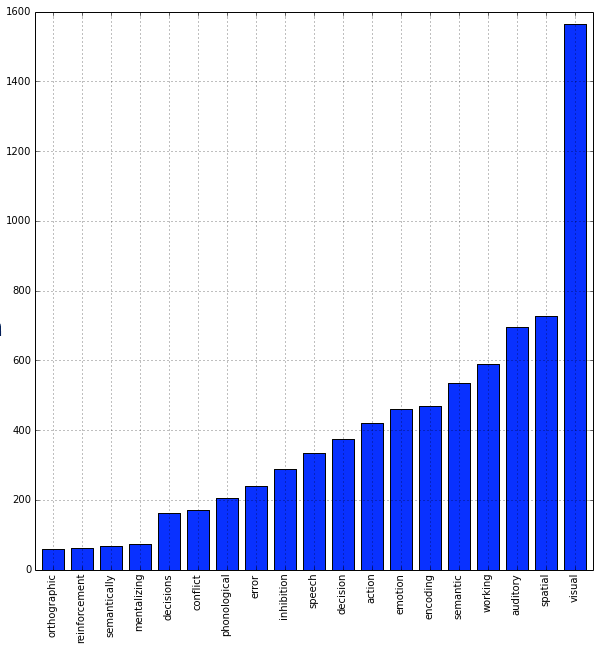
\includegraphics[height=10cm, width=10cm]{histo_new.png}
\end{center}
\caption{\textbf{Distribution of terms across studies:} The x-axis denotes eac term and the y-axis denotes the number of studies in which the term appears.}
\label{fig:histo_new}
\end{figure}

For NeuroVault, the data was not available in a format similar to the openfMRI and NeuroSynth. In this case, we had a total of 17 images, that corresponded to 12 studies. Rather than having the actual labels for these studies, the API provided us with links to online publications corresponding to the study. These were in the \texttt{pdf} format, though in some cases, mutliple formats were also available. We used an approach similar to that already adopted by NeuroSynth, to derive labels for the images. First we converted the \texttt{pdf} formats to plain text using an available python tool~\footnote{http://www.unixuser.org/~euske/python/pdfminer/}. Next we considered a dictionary of terms which we were using for the Neurosynth data and counted how frequently these terms appeared in each study. The final frequency we stored for these terms was normalized by dividing it by the total word count of the document. Thus we ended up with a label representation for each study that was analogous to what was being used in NeuroSynth.


NIPS requires electronic submissions.  The electronic submission site is  
\begin{center}
   \url{http://papers.nips.cc}
\end{center}

Please read carefully the
instructions below, and follow them faithfully.
\subsection{Style}

Papers to be submitted to NIPS 2013 must be prepared according to the
instructions presented here. Papers may be only up to eight pages long,
including figures. Since 2009 an additional ninth page \textit{containing only
cited references} is allowed. Papers that exceed nine pages will not be
reviewed, or in any other way considered for presentation at the conference.
%This is a strict upper bound. 

Please note that this year we have introduced automatic line number generation
into the style file (for \LaTeXe and Word versions). This is to help reviewers
refer to specific lines of the paper when they make their comments. Please do
NOT refer to these line numbers in your paper as they will be removed from the
style file for the final version of accepted papers.

The margins in 2013 are the same as since 2007, which allow for $\approx 15\%$
more words in the paper compared to earlier years. We are also again using 
double-blind reviewing. Both of these require the use of new style files.

Authors are required to use the NIPS \LaTeX{} style files obtainable at the
NIPS website as indicated below. Please make sure you use the current files and
not previous versions. Tweaking the style files may be grounds for rejection.

%% \subsection{Double-blind reviewing}

%% This year we are doing double-blind reviewing: the reviewers will not know 
%% who the authors of the paper are. For submission, the NIPS style file will 
%% automatically anonymize the author list at the beginning of the paper.

%% Please write your paper in such a way to preserve anonymity. Refer to
%% previous work by the author(s) in the third person, rather than first
%% person. Do not provide Web links to supporting material at an identifiable
%% web site.

%%\subsection{Electronic submission}
%%
%% \textbf{THE SUBMISSION DEADLINE IS MAY 31st, 2013. SUBMISSIONS MUST BE LOGGED BY
%% 23:00, MAY 31st, 2013, UNIVERSAL TIME}

%% You must enter your submission in the electronic submission form available at
%% the NIPS website listed above. You will be asked to enter paper title, name of
%% all authors, keyword(s), and data about the contact
%% author (name, full address, telephone, fax, and email). You will need to
%% upload an electronic (postscript or pdf) version of your paper.

%% You can upload more than one version of your paper, until the
%% submission deadline. We strongly recommended uploading your paper in
%% advance of the deadline, so you can avoid last-minute server congestion.
%%
%% Note that your submission is only valid if you get an e-mail
%% confirmation from the server. If you do not get such an e-mail, please
%% try uploading again. 

 \subsection{Multi-Label Prediction}
In addition to reporting the accuracy, we report precision, recall, F1 score and hamming loss. And one correct
\begin{align*}
 \text{Precision} &=\frac{1}{N} \sum_{n=1}^{N} \frac {|S_n \cap \mathcal{Z}_n|}{\mathcal{Z}_n} & \text{Recall}&= \frac{1}{N} \sum_{n=1}^{N} \frac {|S_n \cap \mathcal{Z}_n|}{S_n}\\
 \text{F1 score} &=\frac{1}{N} \sum_{n=1}^{N} \frac{2.0 * Precision_n * Recall_n}{Precision_n + Recall_n} & \text{Hamming loss}&=\frac{1}{N}\sum_{n=1}^{N}\frac{1}{L} |S_n \theta \mathcal{Z}_n |  \\
 \text{Top correct} &=\frac{1}{N} \displaystyle\sum_{n=1}^{N} \mathbb{I}(\mathcal{Z}_{n,max} \in \mathcal{L}_n)& & \\
\end{align*}
$\mathbb{I}$ denotes the indicator function, $S_n$ denotes the true labels  and $\mathcal{Z}_{n,max}$ denotes the label predicted with highest probability for the brain volume $n$. The top correct value is the fraction of the data points on which the model's best predicted label (with maximum probability) was present in the true label set.

This table reports the results of the multilabel classification for the entire label set. Note here that there are $2^{22}$ possible label sets and accuracy is a fairly hard metric to achieve
\begin{table}[h]
\begin{center}
\begin{tabular}{|c|c|c|c|c|c|c|}
\hline
 Model       & Accuracy & Precision & Recall    & F1 score  & Hamming loss & Top correct\\ \hline
 Naive Bayes & 1.3      & \bf{22.36}& \bf{46.04}& \bf{26.63}& 0.207     & 23.7      \\ \hline
 Logistic L1 & 3.2      & 18.92     & 14.16     & 14.53     & 0.111     & 27.9      \\ \hline
 Logistic L2 & \bf{4.1} & 19.58     & 14.73     & 15.22     & 0.108     & \bf{30.0} \\ \hline
 Linear SVM  & 3.7      & 20.34     & 16.40     & 16.24     & 0.115     & 22.5      \\ \hline
 Ward Cluster& 3.4      & 17.53     & 12.99     & 13.43     & \bf{0.107}& 29.8      \\ \hline \hline
 Unique Train$^*$& 0.8      & \bf{33.98}& 22.09     & 24.83     & 0.162     & \bf{36.0} \\ \hline
 All Ones$^*$    & 0.0      & 9.78      & \bf{100.0}& 17.40     & 0.902     & 5.38      \\ \hline
\end{tabular}
\caption{Multilabel classification full tuple results. All values are reported in percentage ($\%$) except hamming loss. Again, excepting for hamming loss where lower loss is better, for all other metrics higher values are better. $^*$Unique Train and All Ones do not use cross validation.}
\end{center}
\end{table}

Overall, while our model does quite poorly on most metrics, this was to be expected given the huge dimensional data, which is also
very sparse. However both SVM as well as $l-2$ regularized logistic regression, do show a relatively good performance on some metrics,
such as the Hamming loss. Most of the models beat the All Ones model on most metrics other than the recall and the Top correct, which 
was to be expected. The model using Ward Clustering shows the best performance for the Hamming Loss metric. Also the Unique train model
does the best on the Top Correct metric, picking out the correct label $36\%$ time.


\subsection{Retrieval of style files}

The style files for NIPS and other conference information are available on the World Wide Web at
\begin{center}
   \url{http://www.nips.cc/}
\end{center}
The file \verb+nips2013.pdf+ contains these 
instructions and illustrates the
various formatting requirements your NIPS paper must satisfy. \LaTeX{}
users can choose between two style files:
\verb+nips11submit_09.sty+ (to be used with \LaTeX{} version 2.09) and
\verb+nips11submit_e.sty+ (to be used with \LaTeX{}2e). The file
\verb+nips2013.tex+ may be used as a ``shell'' for writing your paper. All you
have to do is replace the author, title, abstract, and text of the paper with
your own. The file
\verb+nips2013.rtf+ is provided as a shell for MS Word users.

The formatting instructions contained in these style files are summarized in
sections \ref{gen_inst}, \ref{headings}, and \ref{others} below.

%% \subsection{Keywords for paper submission}
%% Your NIPS paper can be submitted with any of the following keywords (more than one keyword is possible for each paper):

%% \begin{verbatim}
%% Bioinformatics
%% Biological Vision
%% Brain Imaging and Brain Computer Interfacing
%% Clustering
%% Cognitive Science
%% Control and Reinforcement Learning
%% Dimensionality Reduction and Manifolds
%% Feature Selection
%% Gaussian Processes
%% Graphical Models
%% Hardware Technologies
%% Kernels
%% Learning Theory
%% Machine Vision
%% Margins and Boosting
%% Neural Networks
%% Neuroscience
%% Other Algorithms and Architectures
%% Other Applications
%% Semi-supervised Learning
%% Speech and Signal Processing
%% Text and Language Applications

%% \end{verbatim}

\section{General formatting instructions}
\label{gen_inst}

	The text must be confined within a rectangle 5.5~inches (33~picas) wide and
9~inches (54~picas) long. The left margin is 1.5~inch (9~picas).
Use 10~point type with a vertical spacing of 11~points. Times New Roman is the
preferred typeface throughout. Paragraphs are separated by 1/2~line space,
with no indentation.

Paper title is 17~point, initial caps/lower case, bold, centered between
2~horizontal rules. Top rule is 4~points thick and bottom rule is 1~point
thick. Allow 1/4~inch space above and below title to rules. All pages should
start at 1~inch (6~picas) from the top of the page.

%The version of the paper submitted for review should have ``Anonymous Author(s)'' as the author of the paper.

For the final version, authors' names are
set in boldface, and each name is centered above the corresponding
address. The lead author's name is to be listed first (left-most), and
the co-authors' names (if different address) are set to follow. If
there is only one co-author, list both author and co-author side by side.

Please pay special attention to the instructions in section \ref{others}
regarding figures, tables, acknowledgments, and references.

\section{Headings: first level}
\label{headings}

First level headings are lower case (except for first word and proper nouns),
flush left, bold and in point size 12. One line space before the first level
heading and 1/2~line space after the first level heading.

\subsection{Headings: second level}

Second level headings are lower case (except for first word and proper nouns),
flush left, bold and in point size 10. One line space before the second level
heading and 1/2~line space after the second level heading.

\subsubsection{Headings: third level}

Third level headings are lower case (except for first word and proper nouns),
flush left, bold and in point size 10. One line space before the third level
heading and 1/2~line space after the third level heading.

\section{Citations, figures, tables, references}
\label{others}

These instructions apply to everyone, regardless of the formatter being used.

\subsection{Citations within the text}

Citations within the text should be numbered consecutively. The corresponding
number is to appear enclosed in square brackets, such as [1] or [2]-[5]. The
corresponding references are to be listed in the same order at the end of the
paper, in the \textbf{References} section. (Note: the standard
\textsc{Bib\TeX} style \texttt{unsrt} produces this.) As to the format of the
references themselves, any style is acceptable as long as it is used
consistently.

As submission is double blind, refer to your own published work in the 
third person. That is, use ``In the previous work of Jones et al.\ [4]'',
not ``In our previous work [4]''. If you cite your other papers that
are not widely available (e.g.\ a journal paper under review), use
anonymous author names in the citation, e.g.\ an author of the
form ``A.\ Anonymous''. 


\subsection{Footnotes}

Indicate footnotes with a number\footnote{Sample of the first footnote} in the
text. Place the footnotes at the bottom of the page on which they appear.
Precede the footnote with a horizontal rule of 2~inches
(12~picas).\footnote{Sample of the second footnote}

\subsection{Figures}

All artwork must be neat, clean, and legible. Lines should be dark
enough for purposes of reproduction; art work should not be
hand-drawn. The figure number and caption always appear after the
figure. Place one line space before the figure caption, and one line
space after the figure. The figure caption is lower case (except for
first word and proper nouns); figures are numbered consecutively.

Make sure the figure caption does not get separated from the figure.
Leave sufficient space to avoid splitting the figure and figure caption.

You may use color figures. 
However, it is best for the
figure captions and the paper body to make sense if the paper is printed
either in black/white or in color.
\begin{figure}[h]
\begin{center}
%\framebox[4.0in]{$\;$}
%\fbox{\rule[-.5cm]{0cm}{4cm} \rule[-.5cm]{4cm}{0cm}}

\includegraphics[width=2in]{logo.png}
\end{center}
\caption{Sample figure caption.}
\end{figure}

\subsection{Tables}

All tables must be centered, neat, clean and legible. Do not use hand-drawn
tables. The table number and title always appear before the table. See
Table~\ref{sample-table}.

Place one line space before the table title, one line space after the table
title, and one line space after the table. The table title must be lower case
(except for first word and proper nouns); tables are numbered consecutively.

\begin{table}[t]
\caption{Sample table title}
\label{sample-table}
\begin{center}
\begin{tabular}{ll}
\multicolumn{1}{c}{\bf PART}  &\multicolumn{1}{c}{\bf DESCRIPTION}
\\ \hline \\
Dendrite         &Input terminal \\
Axon             &Output terminal \\
Soma             &Cell body (contains cell nucleus) \\
\end{tabular}
\end{center}
\end{table}

\section{Final instructions}
Do not change any aspects of the formatting parameters in the style files.
In particular, do not modify the width or length of the rectangle the text
should fit into, and do not change font sizes (except perhaps in the
\textbf{References} section; see below). Please note that pages should be
numbered.

\section{Preparing PostScript or PDF files}

Please prepare PostScript or PDF files with paper size ``US Letter'', and
not, for example, ``A4''. The -t
letter option on dvips will produce US Letter files.

Fonts were the main cause of problems in the past years. Your PDF file must
only contain Type 1 or Embedded TrueType fonts. Here are a few instructions
to achieve this.

\begin{itemize}

\item You can check which fonts a PDF files uses.  In Acrobat Reader,
select the menu Files$>$Document Properties$>$Fonts and select Show All Fonts. You can
also use the program \verb+pdffonts+ which comes with \verb+xpdf+ and is
available out-of-the-box on most Linux machines.

\item The IEEE has recommendations for generating PDF files whose fonts
are also acceptable for NIPS. Please see
\url{http://www.emfield.org/icuwb2010/downloads/IEEE-PDF-SpecV32.pdf}

\item LaTeX users:

\begin{itemize}

\item Consider directly generating PDF files using \verb+pdflatex+
(especially if you are a MiKTeX user). 
PDF figures must be substituted for EPS figures, however.

\item Otherwise, please generate your PostScript and PDF files with the following commands:
\begin{verbatim} 
dvips mypaper.dvi -t letter -Ppdf -G0 -o mypaper.ps
ps2pdf mypaper.ps mypaper.pdf
\end{verbatim}

Check that the PDF files only contains Type 1 fonts. 
%For the final version, please send us both the Postscript file and
%the PDF file. 

\item xfig "patterned" shapes are implemented with 
bitmap fonts.  Use "solid" shapes instead. 
\item The \verb+\bbold+ package almost always uses bitmap
fonts.  You can try the equivalent AMS Fonts with command
\begin{verbatim}
\usepackage[psamsfonts]{amssymb}
\end{verbatim}
 or use the following workaround for reals, natural and complex: 
\begin{verbatim}
\newcommand{\RR}{I\!\!R} %real numbers
\newcommand{\Nat}{I\!\!N} %natural numbers 
\newcommand{\CC}{I\!\!\!\!C} %complex numbers
\end{verbatim}

\item Sometimes the problematic fonts are used in figures
included in LaTeX files. The ghostscript program \verb+eps2eps+ is the simplest
way to clean such figures. For black and white figures, slightly better
results can be achieved with program \verb+potrace+.
\end{itemize}
\item MSWord and Windows users (via PDF file):
\begin{itemize}
\item Install the Microsoft Save as PDF Office 2007 Add-in from
\url{http://www.microsoft.com/downloads/details.aspx?displaylang=en\&familyid=4d951911-3e7e-4ae6-b059-a2e79ed87041}
\item Select ``Save or Publish to PDF'' from the Office or File menu
\end{itemize}
\item MSWord and Mac OS X users (via PDF file):
\begin{itemize}
\item From the print menu, click the PDF drop-down box, and select ``Save
as PDF...''
\end{itemize}
\item MSWord and Windows users (via PS file):
\begin{itemize}
\item To create a new printer
on your computer, install the AdobePS printer driver and the Adobe Distiller PPD file from
\url{http://www.adobe.com/support/downloads/detail.jsp?ftpID=204} {\it Note:} You must reboot your PC after installing the
AdobePS driver for it to take effect.
\item To produce the ps file, select ``Print'' from the MS app, choose
the installed AdobePS printer, click on ``Properties'', click on ``Advanced.''
\item Set ``TrueType Font'' to be ``Download as Softfont''
\item Open the ``PostScript Options'' folder
\item Select ``PostScript Output Option'' to be ``Optimize for Portability''
\item Select ``TrueType Font Download Option'' to be ``Outline''
\item Select ``Send PostScript Error Handler'' to be ``No''
\item Click ``OK'' three times, print your file.
\item Now, use Adobe Acrobat Distiller or ps2pdf to create a PDF file from
the PS file. In Acrobat, check the option ``Embed all fonts'' if
applicable.
\end{itemize}

\end{itemize}
If your file contains Type 3 fonts or non embedded TrueType fonts, we will
ask you to fix it. 

\subsection{Margins in LaTeX}
 
Most of the margin problems come from figures positioned by hand using
\verb+\special+ or other commands. We suggest using the command
\verb+\includegraphics+
from the graphicx package. Always specify the figure width as a multiple of
the line width as in the example below using .eps graphics
\begin{verbatim}
   \usepackage[dvips]{graphicx} ... 
   \includegraphics[width=0.8\linewidth]{myfile.eps} 
\end{verbatim}
or % Apr 2009 addition
\begin{verbatim}
   \usepackage[pdftex]{graphicx} ... 
   \includegraphics[width=0.8\linewidth]{myfile.pdf} 
\end{verbatim}
for .pdf graphics. 
See section 4.4 in the graphics bundle documentation (\url{http://www.ctan.org/tex-archive/macros/latex/required/graphics/grfguide.ps}) 
 
A number of width problems arise when LaTeX cannot properly hyphenate a
line. Please give LaTeX hyphenation hints using the \verb+\-+ command.


\subsubsection*{Acknowledgments}

Use unnumbered third level headings for the acknowledgments. All
acknowledgments go at the end of the paper. Do not include 
acknowledgments in the anonymized submission, only in the 
final paper. 

\subsubsection*{References}

References follow the acknowledgments. Use unnumbered third level heading for
the references. Any choice of citation style is acceptable as long as you are
consistent. It is permissible to reduce the font size to `small' (9-point) 
when listing the references. {\bf Remember that this year you can use
a ninth page as long as it contains \emph{only} cited references.}

\small{
[1] Alexander, J.A. \& Mozer, M.C. (1995) Template-based algorithms
for connectionist rule extraction. In G. Tesauro, D. S. Touretzky
and T.K. Leen (eds.), {\it Advances in Neural Information Processing
Systems 7}, pp. 609-616. Cambridge, MA: MIT Press.

[2] Bower, J.M. \& Beeman, D. (1995) {\it The Book of GENESIS: Exploring
Realistic Neural Models with the GEneral NEural SImulation System.}
New York: TELOS/Springer-Verlag.

[3] Hasselmo, M.E., Schnell, E. \& Barkai, E. (1995) Dynamics of learning
and recall at excitatory recurrent synapses and cholinergic modulation
in rat hippocampal region CA3. {\it Journal of Neuroscience}
{\bf 15}(7):5249-5262.
}

\end{document}
